
%%%%%%%%%%%%%%%%%%%%%%%%%%%%%%%%%%%%%%%%%%%%%%%%%%%%%%%%%%%%%%%%%%%%%%%%%%%%%%%%%%%

\subsection{Zusammenfassungen und Überblick}\index{Potenzfunktionen!Überblick}

$$y = a\cdot{}x^z$$

$z$ gerade: Gespiegelt an der $y$-Achse

$z$ ungerade: Gespiegelt am Ursprung $O=(0|0)$

Ist ${\color{ForestGreen}a>0}$\TRAINER{ (grün in der Graphik)}, so sind Graphen mit
geraden Exponenten nach oben geöffnet bzw. mit ungeraden Exponenten im
Quadranten I und III.

Ist ${\color{red}a<0}$\TRAINER{ (rot/orange in der Graphik)}, so sind Graphen mit
geraden Exponenten nach unten geöffnet bzw. mit ungeraden Exponenten
im Quadranten II und IV.


\TRAINER{%
  \includegraphics[width=8.5cm]{allg/funktionen/img/potenzfct/potenzFunktionenGerade.png}\hfill{}\includegraphics[width=8.5cm]{allg/funktionen/img/potenzfct/potenzFunktionenUngerade.png}
}%% END Trainer
\noTRAINER{%
  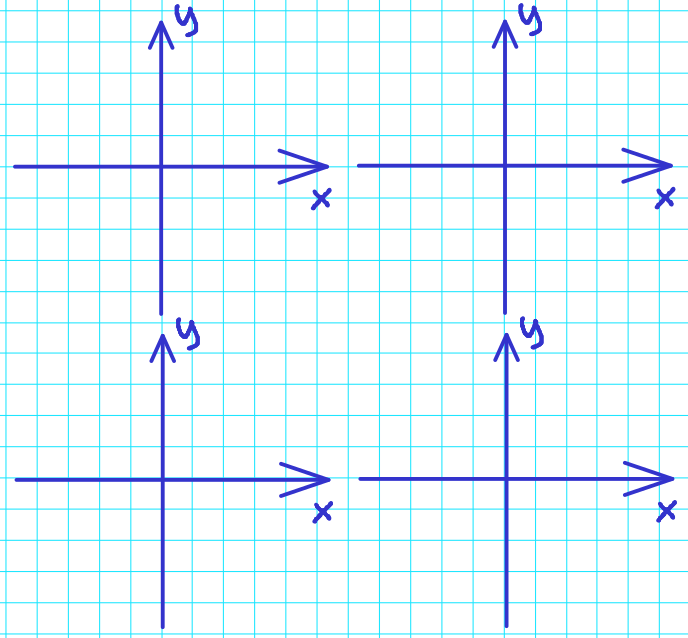
\includegraphics[width=8.5cm]{allg/funktionen/img/potenzfct/potenzFunktionenLeer.png}\hfill{}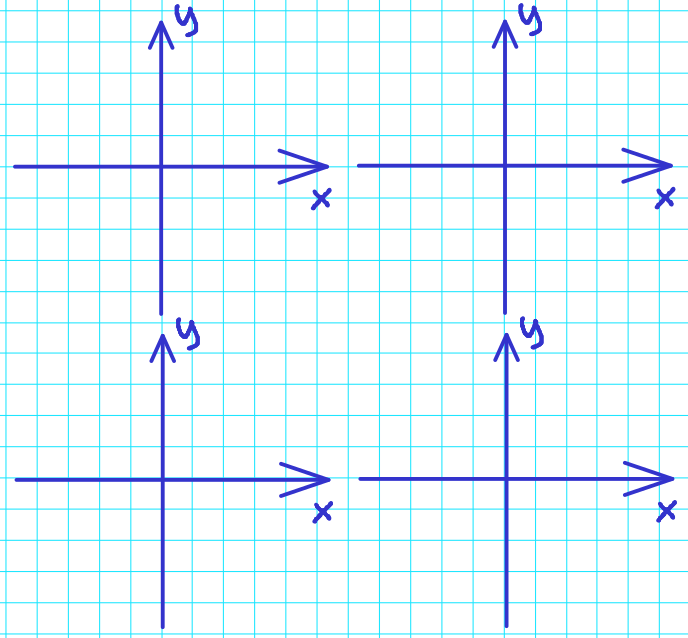
\includegraphics[width=8.5cm]{allg/funktionen/img/potenzfct/potenzFunktionenLeer.png}
}%% END Trainer


\subsection*{Aufgaben}
\AadBMTA{}{25. b) c), 26. a) b), 27. b) c), 33*}

\newpage

